\documentclass[10pt]{article}
\usepackage{amsmath,amssymb,graphicx}
\usepackage{hyperref}

\begin{document}
\title{Test report}
\author{Osian Shelley}


\maketitle
\begin{abstract}
  In this report, we show how to plot a function and its
  derivative. There is nothing particularly difficult about this.
\end{abstract}

\section{Introduction}

Here is an introduction into the problem. We are trying to plot the function
\begin{equation}
  f(x) = \sin(x)
\end{equation}
and its derivative.

\section{Results}

Here are some results. The function is approximated on a grid with
%$N=128$ gripoints. See figure~\ref{fig:func_and_deriv} for results.
%\begin{figure}%
%  \begin{center}
%    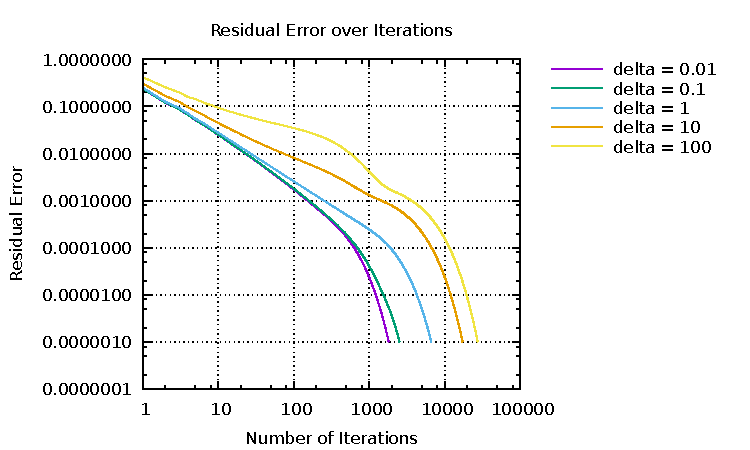
\includegraphics[width=0.49\textwidth]{function}
%    \includegraphics[width=0.49\textwidth]{derivative}
%  \end{center}
%  \caption{This is the figure. Left: Function $f(x)=\sin(x)$. Right:
%    Derivative $f'(x) = \cos(x)$. Note that the $x$-axis shows
%    gridpoint-indices and not the proper $x$ value.
%  \label{fig:func_and_deriv}}
%\end{figure}

\end{document}
